\documentclass[12pt]{report}
\usepackage{amsmath}
\usepackage{amssymb}
\usepackage{graphicx}
\usepackage{hyperref}
\usepackage{color}
\usepackage{float}
\begin{document}
	
	\title{Chromatin Architecture Post UVC damage}
	\maketitle
	\section{Experimental Settings and Findings}
	\begin{enumerate}
		\item Cell type used: U20S, which are human osteosarcoma cells;
		\item H3.3 histones are tagged 48 hours before experiments using the SNAP-tag method, tag color is red;
		\item Repair factors XFP are labeled with GFP;
		\item a region of $20 \mu m^2$ was photo-activated 8-10 hours before UVC;
		\item UVC damage is induced in a region of the cell using a 266 nm laser (0.266 $\mu m$);
		\item Changed to the red fluorescence signal were measured in the entire volume of the cell, post UVC;
		\item Images were acquired using confocal microscopy, with an auto-focus module on, to acquire images from the best focal plane;
		\item Fluorescence intensity were normalized against values measured in undamaged nucleus;
		\item Fluorescence loss at irradiated sites was determined by dividing the intensity in the illuminated area by the intensity of the entire nucleus after background subtraction;
		\item Illuminated area was defined 15 minutes post UVC based on GFP labeled repair factors and was kept similar throughout measurements;
		\item Fluorescent recovery was measured relative to previous illumination starting from the frame with the minimal fluorescent values;
		\item 2D projection of the 3D images were obtained by \textit{maximal intensity z projection}
		\item For sensitivity, most of the cell H3.3 fluorescence was photo-bleached, aside from the region of UVC illumination;
		\item 20\% loss of H3.3 signal from the \textit{entire nucleus} was detected after photo-bleaching the fluorescence patch;
		\item However, using UVC in the fluorescent patch led to 40\% loss of parental H3.3 signal, while no detectable loss was seen in the entire nucleus;		
		\item The depletion of fluorescence in the center of the damage area, 15 minutes post UVC, was accompanied by an increase of density at tits boundary, balancing the loss;
		\item 20\% loss of DNA signal in the damage region, accompanied by an expansion of the region was observed 15 minutes postUVC;
		\item The expansion of the damage region depends on the dose of repair-factor;		
		\item The early repair factor DDB2 recruits histone chaperons HIRA, which promotes the deposition of newly synthesized histones at UVC sites;
		\item newly synthesized histones are detectable in the repair region only 45 minutes post UVC;
		\item Histone chaperons do not participate in histone redestribution after UVC irradiation;
		
	\end{enumerate}
	
	\section{Model and Parameter Estimation}
	For reasons of convenience we will work in units of $100 nm$. Parameter values calculated in the subsection below will be converted to this measure when simulated. 
	
	\subsection{Nucleus Size}
	 Cells' cross-section are 240 $\mu m^2$ in the $x-y$ plane and $11 \mu m$ in height, giving an average radius of $r_c=7.25 \mu m$.  \ref{fig:histoneMarkBeforeDamage}), The red fluorescence represent the histones.
		\begin{figure}[H]
			\centering
			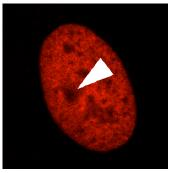
\includegraphics[width=0.2\linewidth]{../histoneMarkBeforeDamage}
			\caption{white triangle represents the UVC damage site, Histones are marked with red}
			\label{fig:histoneMarkBeforeDamage}
		\end{figure}
		
	\subsection{The UV beam}
	UV beam has 3 $\mu m^2$ section, yielding a radius of $r_{uv}=\sqrt{\frac{3}{\pi}}\approx 1 \mu m$. 
	
    \subsection{Histone Density}
		We consider histones to be uniformly distributed in the nucleus and in the damage zone. There are $3\times 10^6$ histones marked, which makes their density $3\times 10^6 /(4 \pi 7.25^3)\approx 630$ histones/$\mu m^3$
		The expected number of histones in the UV beam region is $14.5\pi \times 630\approx 30,000$ histones, assuming the beam is shot through the center of the sphere. 
    
    \subsection{DNA density}
	to be determined	
	
	\subsection{Distribution of damage sites}
	to be determined
	
	\subsection{Defining the region of interest}
	We model the experiment in a region around the damage zone rather than the entire nucleus. We define a region of interest (ROI) in terms of raiuds of the UVC beam radius. The area expanded after UVC occupies $10 \mu m^2$ which gives 3 times the UVC beam radius. We therefore set the radius of the ROI $r_{roi}=3\mu m$.
					    
	\subsection{The chromatin}	
     The chromatin is modeled as a Rouse polymer of $N$ monomers connected by harmonic springs. The dynamics of the polymer is governed by 3 forces: thermal fluctuations, spring force, and bending force.
     Thermal diffusion fluctuation, resulting from the random collision of the polymer with the particles of its surrounding, and is given by 
     \begin{equation*}
     F_d(t) = \sqrt{2D}\frac{dw}{dt}
     \end{equation*}
      with $D$ the diffusion constant, defined by $\frac{k_BT}{\xi}$, $k_B$- the Boltzmann constant, $T$- the absolute temperature in Kelvin, $\xi$-the friction coefficient, and $w$ is a standard white Gaussian noise. 
            
     The spring force, derived from an harmonic potential of springs connecting neighboring monomers, is given by
     \begin{equation*}
      F_e(t) = -\gamma_e\frac{3k_BT}{2b^2}\frac{\partial}{\partial R_n}\sum_{n-1}^{N-1}(|R_n(t)-R_{n+1}(t)| -l_0)^2
     \end{equation*}
     with $\gamma_e>0$ spring constant, $b$- the standard deviation of the distance between monomers, $R_n(t)$ is the 3D position of the $n^{th}$ monomer at time $t$, and $l_0$ is the minimal allowed distance between neighboring monomers.
     
     Bending force on the $n^{th}$ monomer is defined in terms of the angles $\theta_i$ between three adjacent monomers of the chain, $n,n+1,n+2$;
     \begin{equation*}
     F_b(R_n) = -\gamma_b\frac{3k_BT}{2b^2}\frac{\partial}{\partial R_n}\sum_{i=1}^{N-2}(\cos(\theta_i(t))-\cos(\theta_0))^2
     \end{equation*}
               
     The differential equation describing of motion of the chain is thus 
     \begin{equation*}
     \frac{dR_n(t)}{dt}= F_e +F_b +\sqrt{2D} \frac{dw}{dt}     
     \end{equation*}
     
    \subsection{Model Parameters}
      Parameters used in simulations are set proportional to of the quantity $\frac{3k_BT}{b^2}$, which we fix to be 1 by setting the friction factor $\xi=1$. 
    \subsubsection{The parameter b} 
      we set $b=\sqrt{3} \times 100 nm$, 
    \subsection{the minimal distance between monomers -$l_0$}
     We set $l_0$ to be $\sqrt{3}$ to allow fast relaxation of the chain configuration before UVC beam shot. 
    \subsubsection{Number of monomers}
      The number of monomers, $N$, is determined by setting the polymer's radius of gyration to covers the ROI. The radius of gyration is given by $\sqrt{N/6}b$, equating it to $3\mu m$ we get $N\approx 1800$                      
     \subsubsection{The Spring constant}
       We set the spring constant $\gamma_s =1$
     \subsubsection{The bending constant}       
       The bending constant was observed to affect the rate at which the polymer assumes new conformation after UVC damage.
       We set it to be proportional to the bending constant, as $\gamma_b frac{3K_bT}{b^2}$. later we will adjust this constant according to the rate of chromatin expansion seen in experimental data. 
     \subsection{Affected monomers after UVC}
      Affected monomers are those located within the UVC beam at initiation of beam around the center-of-mass of the polymer at that time. Because the polymer assumes random conformation just before beam initiation, it was observed that in many cases there were affected beads for which there were no neighboring affected beads. This phenomena causes peculiarities in the behavior of the chain,and a resting position position could not be found for the affected bead. We, therefore, assign bending force to the affected beads' nearest neighbors to prevent these phenomenas and to form a more continuous segments affected by bending. 
             		
	\section{Simulations}
	
	\subsection{ 3D}
	\subsection{2D}
	
	
	
\end{document}